\documentclass{article}\usepackage[]{graphicx}\usepackage[]{color}
%% maxwidth is the original width if it is less than linewidth
%% otherwise use linewidth (to make sure the graphics do not exceed the margin)
\makeatletter
\def\maxwidth{ %
  \ifdim\Gin@nat@width>\linewidth
    \linewidth
  \else
    \Gin@nat@width
  \fi
}
\makeatother

\definecolor{fgcolor}{rgb}{0.345, 0.345, 0.345}
\newcommand{\hlnum}[1]{\textcolor[rgb]{0.686,0.059,0.569}{#1}}%
\newcommand{\hlstr}[1]{\textcolor[rgb]{0.192,0.494,0.8}{#1}}%
\newcommand{\hlcom}[1]{\textcolor[rgb]{0.678,0.584,0.686}{\textit{#1}}}%
\newcommand{\hlopt}[1]{\textcolor[rgb]{0,0,0}{#1}}%
\newcommand{\hlstd}[1]{\textcolor[rgb]{0.345,0.345,0.345}{#1}}%
\newcommand{\hlkwa}[1]{\textcolor[rgb]{0.161,0.373,0.58}{\textbf{#1}}}%
\newcommand{\hlkwb}[1]{\textcolor[rgb]{0.69,0.353,0.396}{#1}}%
\newcommand{\hlkwc}[1]{\textcolor[rgb]{0.333,0.667,0.333}{#1}}%
\newcommand{\hlkwd}[1]{\textcolor[rgb]{0.737,0.353,0.396}{\textbf{#1}}}%
\let\hlipl\hlkwb

\usepackage{framed}
\makeatletter
\newenvironment{kframe}{%
 \def\at@end@of@kframe{}%
 \ifinner\ifhmode%
  \def\at@end@of@kframe{\end{minipage}}%
  \begin{minipage}{\columnwidth}%
 \fi\fi%
 \def\FrameCommand##1{\hskip\@totalleftmargin \hskip-\fboxsep
 \colorbox{shadecolor}{##1}\hskip-\fboxsep
     % There is no \\@totalrightmargin, so:
     \hskip-\linewidth \hskip-\@totalleftmargin \hskip\columnwidth}%
 \MakeFramed {\advance\hsize-\width
   \@totalleftmargin\z@ \linewidth\hsize
   \@setminipage}}%
 {\par\unskip\endMakeFramed%
 \at@end@of@kframe}
\makeatother

\definecolor{shadecolor}{rgb}{.97, .97, .97}
\definecolor{messagecolor}{rgb}{0, 0, 0}
\definecolor{warningcolor}{rgb}{1, 0, 1}
\definecolor{errorcolor}{rgb}{1, 0, 0}
\newenvironment{knitrout}{}{} % an empty environment to be redefined in TeX

\usepackage{alltt}


\documentclass[english]{article}
\usepackage[utf8]{inputenc}
\usepackage[margin=1.8cm,a4paper]{geometry}
\usepackage[english]{babel} % hyphenation
\usepackage{csquotes}
\usepackage{amsmath,amssymb,amsthm} % for mathematical
\usepackage{graphicx} % to include graphics
\newcommand{\myparagraph}[1]{\paragraph{#1}\mbox{}\\}


%%Bib Setup:
\usepackage[style=apa, sorting=nyt, backend=biber, maxcitenames=2, useprefix=true, doi=false, isbn=false, natbib=true, language=american]{biblatex}
\DeclareLanguageMapping{american}{american-apa}
\newcommand*{\bibtitle}{Works Cited}
\addbibresource{references.bib}

%%In-text \Sexpr{} setup for lmer:
\newcommand{\betavec}{\beta = }
\newcommand{\betavec}{{\bm\beta}}
\newcommand{\CIstart}{(95\% CI =}
\newcommand{\CIfinish}{),}
\newcommand{\SE}{SE =}
\newcommand{\pvalue}{p =}
\newcommand{\MR2}{marginal R^2 =}
\newcommand{\CR2}{conditional R^2 =}
% Wald statistic for normality of residuals:
\newcommand{\resdist}{W = }
% Cook's Distances (influential cases)
\newcommand{\cooksD}{Cook's Distances}

% setting global settings and loading useful libraries
\title{Field Experiment}
\date{}
\author{Jacob Taylor & Emma Cohen \\ Institute of Cognitive \and Evolutionary Anthropology, University of Oxford}
\IfFileExists{upquote.sty}{\usepackage{upquote}}{}
\begin{document}
\maketitle
\begin{knitrout}
\definecolor{shadecolor}{rgb}{0.969, 0.969, 0.969}\color{fgcolor}\begin{kframe}


{\ttfamily\noindent\bfseries\color{errorcolor}{\#\# Error in contrib.url(repos, "{}source"{}): trying to use CRAN without setting a mirror}}

{\ttfamily\noindent\itshape\color{messagecolor}{\#\# Loading required package: Matrix}}

{\ttfamily\noindent\bfseries\color{errorcolor}{\#\# Error in contrib.url(repos, "{}source"{}): trying to use CRAN without setting a mirror}}\end{kframe}
\end{knitrout}









\begin{knitrout}
\definecolor{shadecolor}{rgb}{0.969, 0.969, 0.969}\color{fgcolor}

{\centering 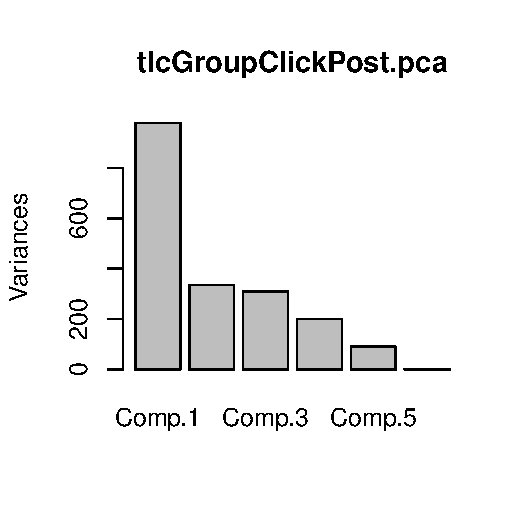
\includegraphics[width=\maxwidth]{figure/dataReductionGroupClickPost-1} 

}



\end{knitrout}



%MODEL:






A LMER was used to model the relationship between group performance expectation violations and group click.  Group Performance Expectations, Condition, and their interaction were included as fixed effects, and experiment session was modelled as a random effect (intercept and slope).  To control for perceptions of individual performance relative to prior expectations, post-Experiment arousal, the average performance outcome of each invasion drill trial, and subjective and objective measures of athlete technical competence, these factors were included as fixed effects.

The model revealed a significant positive main effect of group performance expectation violation on feelings of team click with the training group,
  \betavec
  
  0.4194001
  %groupPerfExpClick.controls.tidy[2,2].

\end{document}





